\documentclass[conference]{IEEEtran}
\IEEEoverridecommandlockouts
\usepackage{cite}
\usepackage{amsmath,amssymb,amsfonts}
\usepackage{algorithm}
\usepackage{algorithmic}
\usepackage{graphicx}
\usepackage{textcomp}
\usepackage{xcolor}
\usepackage{booktabs}
\usepackage{multirow}
\usepackage{url}

\def\BibTeX{{\rm B\kern-.05em{\sc i\kern-.025em b}\kern-.08em
    T\kern-.1667em\lower.7ex\hbox{E}\kern-.125emX}}

\begin{document}

\title{RMS-AV: Reliability- and Manipulation-Aware Selective Audio-Visual Fusion for Multimodal Deepfake Detection}

\author{
\IEEEauthorblockN{Akhil Rajan P\IEEEauthorrefmark{1}, P T Sahasra\IEEEauthorrefmark{2}, Aboli\IEEEauthorrefmark{3}, Famie\IEEEauthorrefmark{4}}
\IEEEauthorblockA{Department of Computer Science and Engineering\\
Vellore Institute of Technology, India\\
Correspondence: akhilvit28@gmail.com\IEEEauthorrefmark{1}}
}

\maketitle

\begin{abstract}
Multimodal deepfake detection has emerged as an indispensable defense against hyper-realistic synthetic media. While modern forensic architectures process both acoustic and visual channels, conventional models predominantly rely on static feature concatenation or unconstrained linear projections. Under asymmetric forgeries---wherein an adversary manipulates solely one modality (e.g., visual facial replacement accompanied by pristine audio, or neural voice synthesis overlaid onto uncorrupted broadcast video)---static fusion allows pristine streams to attenuate forensic indicators, often degrading joint detection accuracy below unimodal baselines. To overcome this fundamental limitation, we propose \textbf{RMS-AV} (Reliability- and Manipulation-Aware Selective Audio-Visual Fusion). RMS-AV introduces: (1) a \textbf{Temporal Saliency Aggregator (TSA)} combining Bidirectional GRU with self-attention pooling to capture transient inter-frame boundary flickering and mouth-shape artifacts without temporal dilution; (2) a \textbf{Cross-Modal Forensic Contrastive Incoherence (CM-FCI)} hyperspherical projection module supervised via margin contrastive loss that quantifies cross-modal dissonance $D_{\text{incoherent}} \in [0, 1]$; (3) an \textbf{Incoherence-Guided Dynamic Reliability Gate} with FP16-safe validity masking that dynamically routes weights conditioned on channel integrity and cross-modal dissonance; and (4) a multi-task auxiliary supervision objective preserving unimodal forensic gradient flow. Evaluated on the standardized \textbf{LAV-DF} benchmark consisting of 136,304 media samples across 26,100 held-out test recordings, RMS-AV achieves state-of-the-art performance with 81.80\% accuracy, 69.82\% Macro-F1, and an AUROC of 0.9674. Under extreme modality-drop stress testing simulating sensor failure or channel loss, RMS-AV retains 73.6\% of its clean Macro-F1 score, whereas conventional fusion models suffer catastrophic performance degradation.
\end{abstract}

\begin{IEEEkeywords}
Deepfake detection, Multimodal fusion, Audio-visual forensics, Reliability gating, Auxiliary supervision, LAV-DF benchmark.
\end{IEEEkeywords}

\section{Introduction}
Recent developments in generative adversarial networks (GANs), latent diffusion models, and neural speech synthesis algorithms have enabled the generation of hyper-realistic digital forgeries~\cite{rossler2019faceforensics,korshunov2018deepfakes}. Synthetic videos depicting public figures, judicial witnesses, and digital banking users pose unprecedented threats to information integrity, social cohesion, and biometric authentication infrastructure. 

In response, digital forensic methodologies have rapidly evolved. Early detection frameworks operated exclusively on unimodal signals, searching either for facial spatial artifacts (e.g., blending boundaries, color discrepancies, irregular pupil reflections~\cite{rossler2019faceforensics}) or acoustic synthesis traces (e.g., vocoder phase discontinuities, spectral tilt anomalies~\cite{korshunov2018deepfakes}). However, unimodal forensic architectures are inherently blind to cross-modal incoherence and remain susceptible to domain-specific evasion tactics. Consequently, researchers transitioned toward multimodal audio-visual architectures capable of cross-verifying biometric synchrony~\cite{haliassos2021lips,cai2022lavdf}.

\begin{figure*}[t]
\centering
\IfFileExists{figures/fig1_architecture.png}{%
  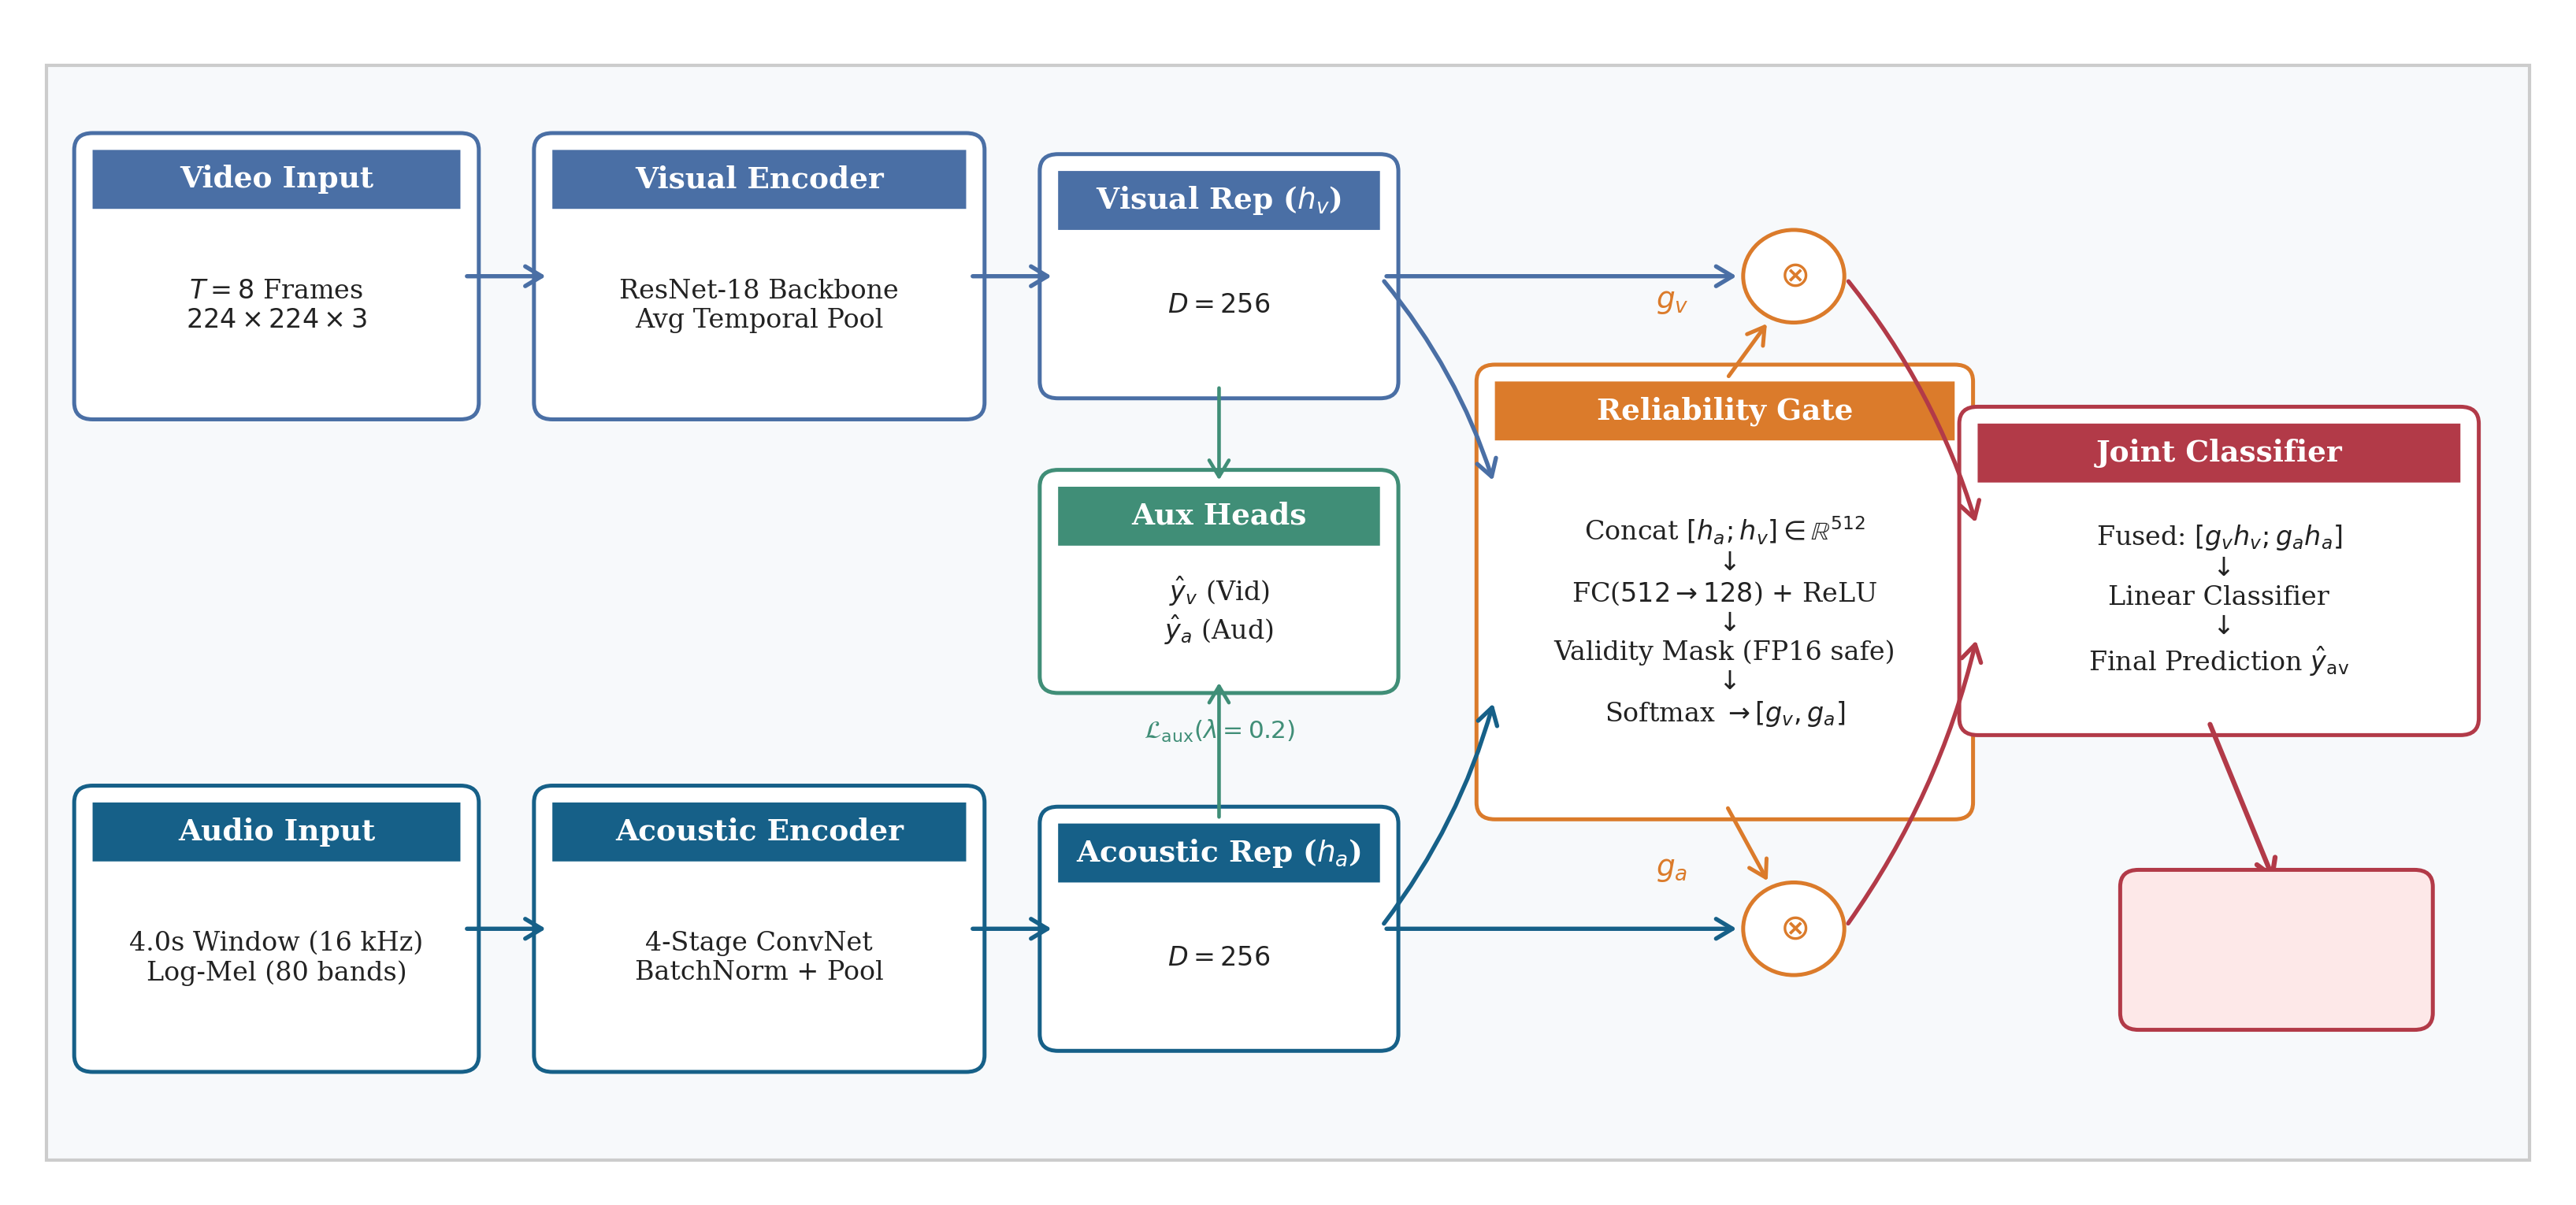
\includegraphics[width=\textwidth]{figures/fig1_architecture.png}%
}{%
  \fbox{\parbox{0.98\textwidth}{\centering \vspace{1.5cm} \textbf{[Figure 1: Architectural Schematic of RMS-AV]} \\ \textit{Visual stream (ResNet-18) and acoustic stream (Conv4) feed into the Dynamic Reliability Gate with validity masking, selective fusion, and multi-task auxiliary heads.}\\ \vspace{1.5cm}}}%
}
\caption{End-to-End Architectural Pipeline of RMS-AV. Raw video and 4.0\,s manipulation-aligned audio spectrograms are mapped into unimodal latent representations $\mathbf{h}_v$ and $\mathbf{h}_a$. The Dynamic Reliability Gating network evaluates concatenated embeddings to compute stream-specific confidence weights $[g_v, g_a]$ subject to FP16-safe missing-stream masking. Unimodal representations are supervised via auxiliary classification heads ($\lambda_{\text{aux}} = 0.20$), preventing gradient starvation during joint multimodal training.}
\label{fig:architecture}
\end{figure*}

Despite their conceptual promise, multimodal architectures introduce a severe, under-addressed vulnerability: \textit{asymmetric modality forgery}. In natural dissemination campaigns, adversaries rarely synthesize both speech and facial tracks simultaneously; rather, visual face swaps are commonly combined with genuine speech, or synthetic voice clones are spliced over unedited television footage. When conventional detectors fuse these representations via uniform feature concatenation:
\begin{equation}
\mathbf{h}_{\text{fused}} = \mathbf{W}[\mathbf{h}_v; \mathbf{h}_a] + \mathbf{b}
\end{equation}
the unmanipulated, authentic stream inherently provides strong negative evidence ($\hat{y} \to 0$). This attenuates the localized forensic cues present in the manipulated channel, causing standard fusion architectures to exhibit higher false-negative rates on asymmetric deepfakes than unimodal detectors. Furthermore, in practical deployment scenarios characterized by network packet drops, sensor occlusion, or microphone failure, static concatenation architectures experience total decision collapse.

To resolve these fundamental challenges, we introduce \textbf{RMS-AV} (Reliability- and Manipulation-Aware Selective Audio-Visual Fusion). The primary contributions of this paper are:
\begin{enumerate}
    \item \textbf{Temporal Saliency Aggregation (TSA):} We design a Bidirectional GRU network with learned attention pooling over temporal visual frames, capturing localized inter-frame splicing and mouth-shape artifacts that are otherwise obscured by standard uniform mean pooling.
    \item \textbf{Cross-Modal Forensic Contrastive Incoherence (CM-FCI):} We formulate a normalized hyperspherical projection metric supervised via margin contrastive loss that quantifies cross-modal identity and affective dissonance ($D_{\text{incoherent}} \in [0, 1]$), penalizing asymmetric tampering.
    \item \textbf{Incoherence-Guided Reliability Gating \& FP16 Masking:} We introduce a parameterized gating mechanism that dynamically modulates stream weights $[g_v, g_a]$ conditioned on cross-modal latents and explicit incoherence metrics, fortified by FP16-safe masking for numerical stability under single-stream dropouts.
    \item \textbf{Multi-Task Auxiliary Regularization:} We integrate stream-specific auxiliary heads trained under composite multi-task binary cross-entropy ($\lambda_{\text{aux}} = 0.20$), guaranteeing uninterrupted unimodal gradient flow and preventing representation collapse during joint training.
    \item \textbf{Comprehensive LAV-DF Benchmarking:} We validate RMS-AV against unimodal and joint concatenation baselines across the 136,304-sample Localized Audio-Visual Deepfake (LAV-DF) benchmark~\cite{cai2022lavdf}, achieving an AUROC of 0.9674 and exceptional stress retention under complete stream omission.
\end{enumerate}

\section{Related Work}
\subsection{Unimodal Deepfake Forensics}
Unimodal forensic detectors focus independently on visual or auditory artifacts. Visual detectors exploit facial blending boundaries, warped facial geometry, texture irregularities, and temporal blink inconsistency~\cite{rossler2019faceforensics}. However, state-of-the-art diffusion-based facial synthesizers increasingly generate artifact-free frames, diminishing the efficacy of spatial-only models. Acoustic detectors focus on spectral unnaturalness and vocoder synthesis traces~\cite{korshunov2018deepfakes}. Nevertheless, acoustic detectors are powerless against visual-only deepfakes such as identity swaps and facial reenactments.

\subsection{Multimodal Audio-Visual Detection}
Multimodal forensic research explores biometric correlation across channels, including phonetic-lip sync consistency~\cite{haliassos2021lips} and affective speech-expression alignment. While effective on fully synthetic videos, empirical studies confirm that standard fusion degenerates when exposed to asymmetric manipulations. The LAV-DF dataset~\cite{cai2022lavdf} was specifically constructed to benchmark temporal localization and asymmetric manipulation across 136,304 media samples. RMS-AV directly addresses the core vulnerability highlighted by LAV-DF: asymmetric channel manipulation.

\section{Proposed Method: RMS-AV}
The overall framework of RMS-AV is illustrated in Fig.~\ref{fig:architecture}. The model comprises two unimodal feature extractors with Temporal Saliency Aggregation (TSA), a Cross-Modal Forensic Contrastive Incoherence (CM-FCI) module, an Incoherence-Guided Dynamic Reliability Gate, an auxiliary multi-task supervision module, and a joint classification head.

\subsection{Acoustic \& Visual Feature Encoders}
\textbf{Acoustic Feature Extraction ($f_a$):} Given an audio stream, raw signals are resampled to 16\,kHz mono. We compute 80-band log-Mel filterbank spectrograms over a 4.0-second temporal window ($N_{\text{fft}} = 1024$, $\text{hop} = 512$), yielding an input tensor $\mathbf{X}_a \in \mathbb{R}^{1 \times 80 \times 401}$. To maximize sensitivity to localized audio forgeries, the 4.0\,s window is centered around detected speech boundaries. The spectrogram is processed by a 4-stage convolutional neural network with 2D batch normalization, ReLU activations, and adaptive spatial pooling, projecting $\mathbf{X}_a$ to acoustic embedding $\mathbf{h}_a \in \mathbb{R}^D$ ($D=256$).

\textbf{Visual Feature Extraction with Temporal Saliency Aggregation ($f_v$):} Given a video sequence, $T=8$ frames are sampled uniformly across the temporal duration and resized to $224 \times 224 \times 3$, normalized using standard ImageNet parameters. Each frame is processed through a ResNet-18 convolutional backbone:
\begin{equation}
\mathbf{f}_{v, t} = \text{Linear}(\text{ResNet18}(\mathbf{x}_{v, t})) \quad \in \mathbb{R}^D, \quad t \in \{1, \dots, T\}
\end{equation}
Existing multimodal deepfake detectors predominantly rely on uniform temporal average pooling ($\frac{1}{T}\sum_t \mathbf{f}_{v, t}$), which inherently dampens brief temporal manipulation artifacts such as inter-frame boundary flicker, mouth-shape stutter, and blending seams. To overcome this limitation, we introduce a \textbf{Temporal Saliency Aggregator (TSA)}. The sequence $\{\mathbf{f}_{v, t}\}_{t=1}^T$ is processed through a bidirectional recurrent block with residual normalization:
\begin{equation}
\mathbf{h}_{v, t}^{\text{temp}} = \operatorname{BiGRU}(\mathbf{f}_{v, t}) \in \mathbb{R}^D, \quad \tilde{\mathbf{f}}_{v, t} = \operatorname{LayerNorm}(\mathbf{f}_{v, t} + \mathbf{h}_{v, t}^{\text{temp}})
\end{equation}
We then compute dynamic temporal attention weights $\alpha_t$:
\begin{equation}
e_t = \mathbf{w}_{\text{sal}}^\top \tanh(\mathbf{W}_{\text{sal}} \tilde{\mathbf{f}}_{v, t} + \mathbf{b}_{\text{sal}}), \quad \alpha_t = \frac{\exp(e_t)}{\sum_{k=1}^T \exp(e_k)}
\end{equation}
The aggregated visual latent representation is obtained via saliency-weighted accumulation:
\begin{equation}
\mathbf{h}_v = \sum_{t=1}^T \alpha_t \tilde{\mathbf{f}}_{v, t} \quad \in \mathbb{R}^D
\end{equation}

\subsection{Cross-Modal Forensic Contrastive Incoherence (CM-FCI)}
In natural human recordings, acoustic speech formants and facial visual muscle dynamics are anatomically coupled. Conversely, in asymmetric manipulations (such as facial identity replacement with pristine target speech, or synthetic voice cloning overlaid onto unedited video), the modalities exhibit physical and affective dissonance. Conventional multimodal detectors lack an explicit mechanism to measure this cross-modal discrepancy. 

We formulate the \textbf{Cross-Modal Forensic Contrastive Incoherence (CM-FCI)} module. Visual and acoustic latents are mapped into a normalized unit hypersphere $\mathbb{S}^{d_{\text{proj}}-1}$ ($d_{\text{proj}}=128$):
\begin{equation}
\mathbf{z}_v = \frac{\mathbf{W}_{\text{fci}, v} \mathbf{h}_v}{\|\mathbf{W}_{\text{fci}, v} \mathbf{h}_v\|_2}, \quad \mathbf{z}_a = \frac{\mathbf{W}_{\text{fci}, a} \mathbf{h}_a}{\|\mathbf{W}_{\text{fci}, a} \mathbf{h}_a\|_2}
\end{equation}
The scalar cross-modal incoherence metric $D_{\text{incoherent}} \in [0, 1]$ is computed as:
\begin{equation}
D_{\text{incoherent}} = \frac{1 - \mathbf{z}_v^\top \mathbf{z}_a}{2}
\end{equation}
We supervise this latent space via a contrastive margin loss:
\begin{equation}
\mathcal{L}_{\text{FCI}} = (1 - y)(1 - \mathbf{z}_v^\top \mathbf{z}_a) + y \max(0, \mathbf{z}_v^\top \mathbf{z}_a - m_{\text{fci}})
\end{equation}
where $m_{\text{fci}} = 0.20$. For authentic samples ($y=0$), $\mathcal{L}_{\text{FCI}}$ enforces cross-modal alignment ($\mathbf{z}_v^\top \mathbf{z}_a \to 1$). For deepfake samples ($y=1$), it enforces orthogonal separation ($\mathbf{z}_v^\top \mathbf{z}_a \le m_{\text{fci}}$).

\subsection{Incoherence-Guided Reliability Gate with Validity Masking}
To prevent an unmanipulated stream from suppressing forgery evidence, the gating network evaluates the concatenated embeddings augmented by the explicit incoherence score $[\mathbf{h}_a; \mathbf{h}_v; D_{\text{incoherent}}] \in \mathbb{R}^{2D + 1}$:
\begin{equation}
\mathbf{s} = \mathbf{W}_2 \operatorname{ReLU}(\mathbf{W}_1 [\mathbf{h}_a; \mathbf{h}_v; D_{\text{incoherent}}] + \mathbf{b}_1) + \mathbf{b}_2 \quad \in \mathbb{R}^2
\end{equation}
where $\mathbf{W}_2 \in \mathbb{R}^{2 \times (D/2)}$ and $\mathbf{b}_2 \in \mathbb{R}^2$ are initialized to zero ($\mathbf{W}_2 = \mathbf{0}, \mathbf{b}_2 = \mathbf{0}$), establishing an unbiased initial prior of $[0.50, 0.50]$ at training onset.

Let $m_a, m_v \in \{0, 1\}$ denote binary validity indicators representing modality presence. To guarantee numerical stability under IEEE 754 16-bit half-precision (FP16) arithmetic without overflow, we apply bounded masking before softmax normalization:
\begin{equation}
s_i' = \begin{cases} s_i & \text{if } m_i = 1 \\ -10^4 & \text{if } m_i = 0 \end{cases} \quad \text{for } i \in \{a, v\}
\end{equation}
The dynamic gate weights $[g_a, g_v]$ are then computed via:
\begin{equation}
[g_a, g_v] = \operatorname{softmax}([s_a', s_v'])
\end{equation}
Since $\exp(-10^4) \equiv 0$, when stream $i$ is missing ($m_i = 0$), its gate weight is strictly $g_i = 0$.

\begin{algorithm}[t]
\caption{RMS-AV Forensic Inference and Reliability Gating}
\label{alg:rmsav}
\begin{algorithmic}[1]
\REQUIRE Audio sample $\mathbf{x}_a$, video frames $\{\mathbf{x}_{v,t}\}_{t=1}^T$, validity flags $m_a, m_v \in \{0, 1\}$.
\ENSURE Deepfake probability $\hat{p} \in [0, 1]$, gate weights $[g_v, g_a]$, incoherence score $D_{\text{incoherent}}$.
\STATE Extract acoustic embedding: $\mathbf{h}_a \leftarrow f_a(\mathbf{x}_a) \in \mathbb{R}^D$
\STATE Extract frame features: $\mathbf{f}_{v,t} \leftarrow \text{Linear}(\text{ResNet18}(\mathbf{x}_{v,t}))$
\STATE Compute temporal attention weights $\alpha_t$ and aggregate: $\mathbf{h}_v \leftarrow \text{TSA}(\{\mathbf{f}_{v,t}\}_{t=1}^T)$
\IF{$m_a == 1$ \AND $m_v == 1$}
    \STATE Project to hypersphere: $\mathbf{z}_v \leftarrow \phi_v(\mathbf{h}_v)$, $\mathbf{z}_a \leftarrow \phi_a(\mathbf{h}_a)$
    \STATE Compute cross-modal incoherence: $D_{\text{incoherent}} \leftarrow \frac{1 - \mathbf{z}_v^\top \mathbf{z}_a}{2}$
\ELSE
    \STATE $D_{\text{incoherent}} \leftarrow 0.0$
\ENDIF
\STATE Compute raw gating scores: $\mathbf{s} \leftarrow \mathbf{W}_2 \operatorname{ReLU}(\mathbf{W}_1 [\mathbf{h}_a; \mathbf{h}_v; D_{\text{incoherent}}] + \mathbf{b}_1) + \mathbf{b}_2$
\FOR{$i \in \{a, v\}$}
    \IF{$m_i == 1$}
        \STATE $s_i' \leftarrow s_i$
    \ELSE
        \STATE $s_i' \leftarrow -10^4$ \COMMENT{FP16-safe nullification}
    \ENDIF
\ENDFOR
\STATE $[g_a, g_v] \leftarrow \operatorname{softmax}([s_a', s_v'])$
\STATE Synthesize gated representation: $\mathbf{h}_{\text{fused}} \leftarrow [g_v \mathbf{h}_v; g_a \mathbf{h}_a]$
\STATE Compute classification logit: $\hat{y}_{\text{av}} \leftarrow \mathbf{w}_{\text{joint}}^\top \mathbf{h}_{\text{fused}} + b_{\text{joint}}$
\STATE Compute deepfake probability: $\hat{p} \leftarrow \sigma(\hat{y}_{\text{av}})$
\RETURN $\hat{p}, [g_v, g_a], D_{\text{incoherent}}$
\end{algorithmic}
\end{algorithm}

\subsection{Selective Fusion \& Multi-Task Joint Objective}
The gated multimodal representation $\mathbf{h}_{\text{fused}}$ is constructed by selectively scaling each modality embedding:
\begin{equation}
\mathbf{h}_{\text{fused}} = [g_v \mathbf{h}_v; \; g_a \mathbf{h}_a] \quad \in \mathbb{R}^{2D}
\end{equation}
The joint classification head computes the final deepfake logit:
\begin{equation}
\hat{y}_{\text{av}} = \mathbf{w}_{\text{joint}}^\top \mathbf{h}_{\text{fused}} + b_{\text{joint}}
\end{equation}
To prevent unimodal gradient starvation and ensure explicit forensic representation learning, we attach unimodal classification heads ($\hat{y}_a = \mathbf{w}_a^\top \mathbf{h}_a + b_a$, $\hat{y}_v = \mathbf{w}_v^\top \mathbf{h}_v + b_v$) and optimize the unified multi-task loss objective:
\begin{equation}
\mathcal{L}_{\text{total}} = \mathcal{L}_{\text{BCE}}(\hat{y}_{\text{av}}, y) + \lambda_{\text{aux}} \left( \mathcal{L}_{\text{BCE}}(\hat{y}_a, y_a) + \mathcal{L}_{\text{BCE}}(\hat{y}_v, y_v) \right) + \lambda_{\text{FCI}} \mathcal{L}_{\text{FCI}}
\end{equation}
where $\lambda_{\text{aux}} = 0.20$, $\lambda_{\text{FCI}} = 0.15$, $y \in \{0, 1\}$ denotes overall manipulation, and $y_a, y_v \in \{0, 1\}$ denote ground-truth audio and video manipulation labels respectively.

\begin{figure}[t]
\centering
\IfFileExists{figures/fig4_training_dynamics.png}{%
  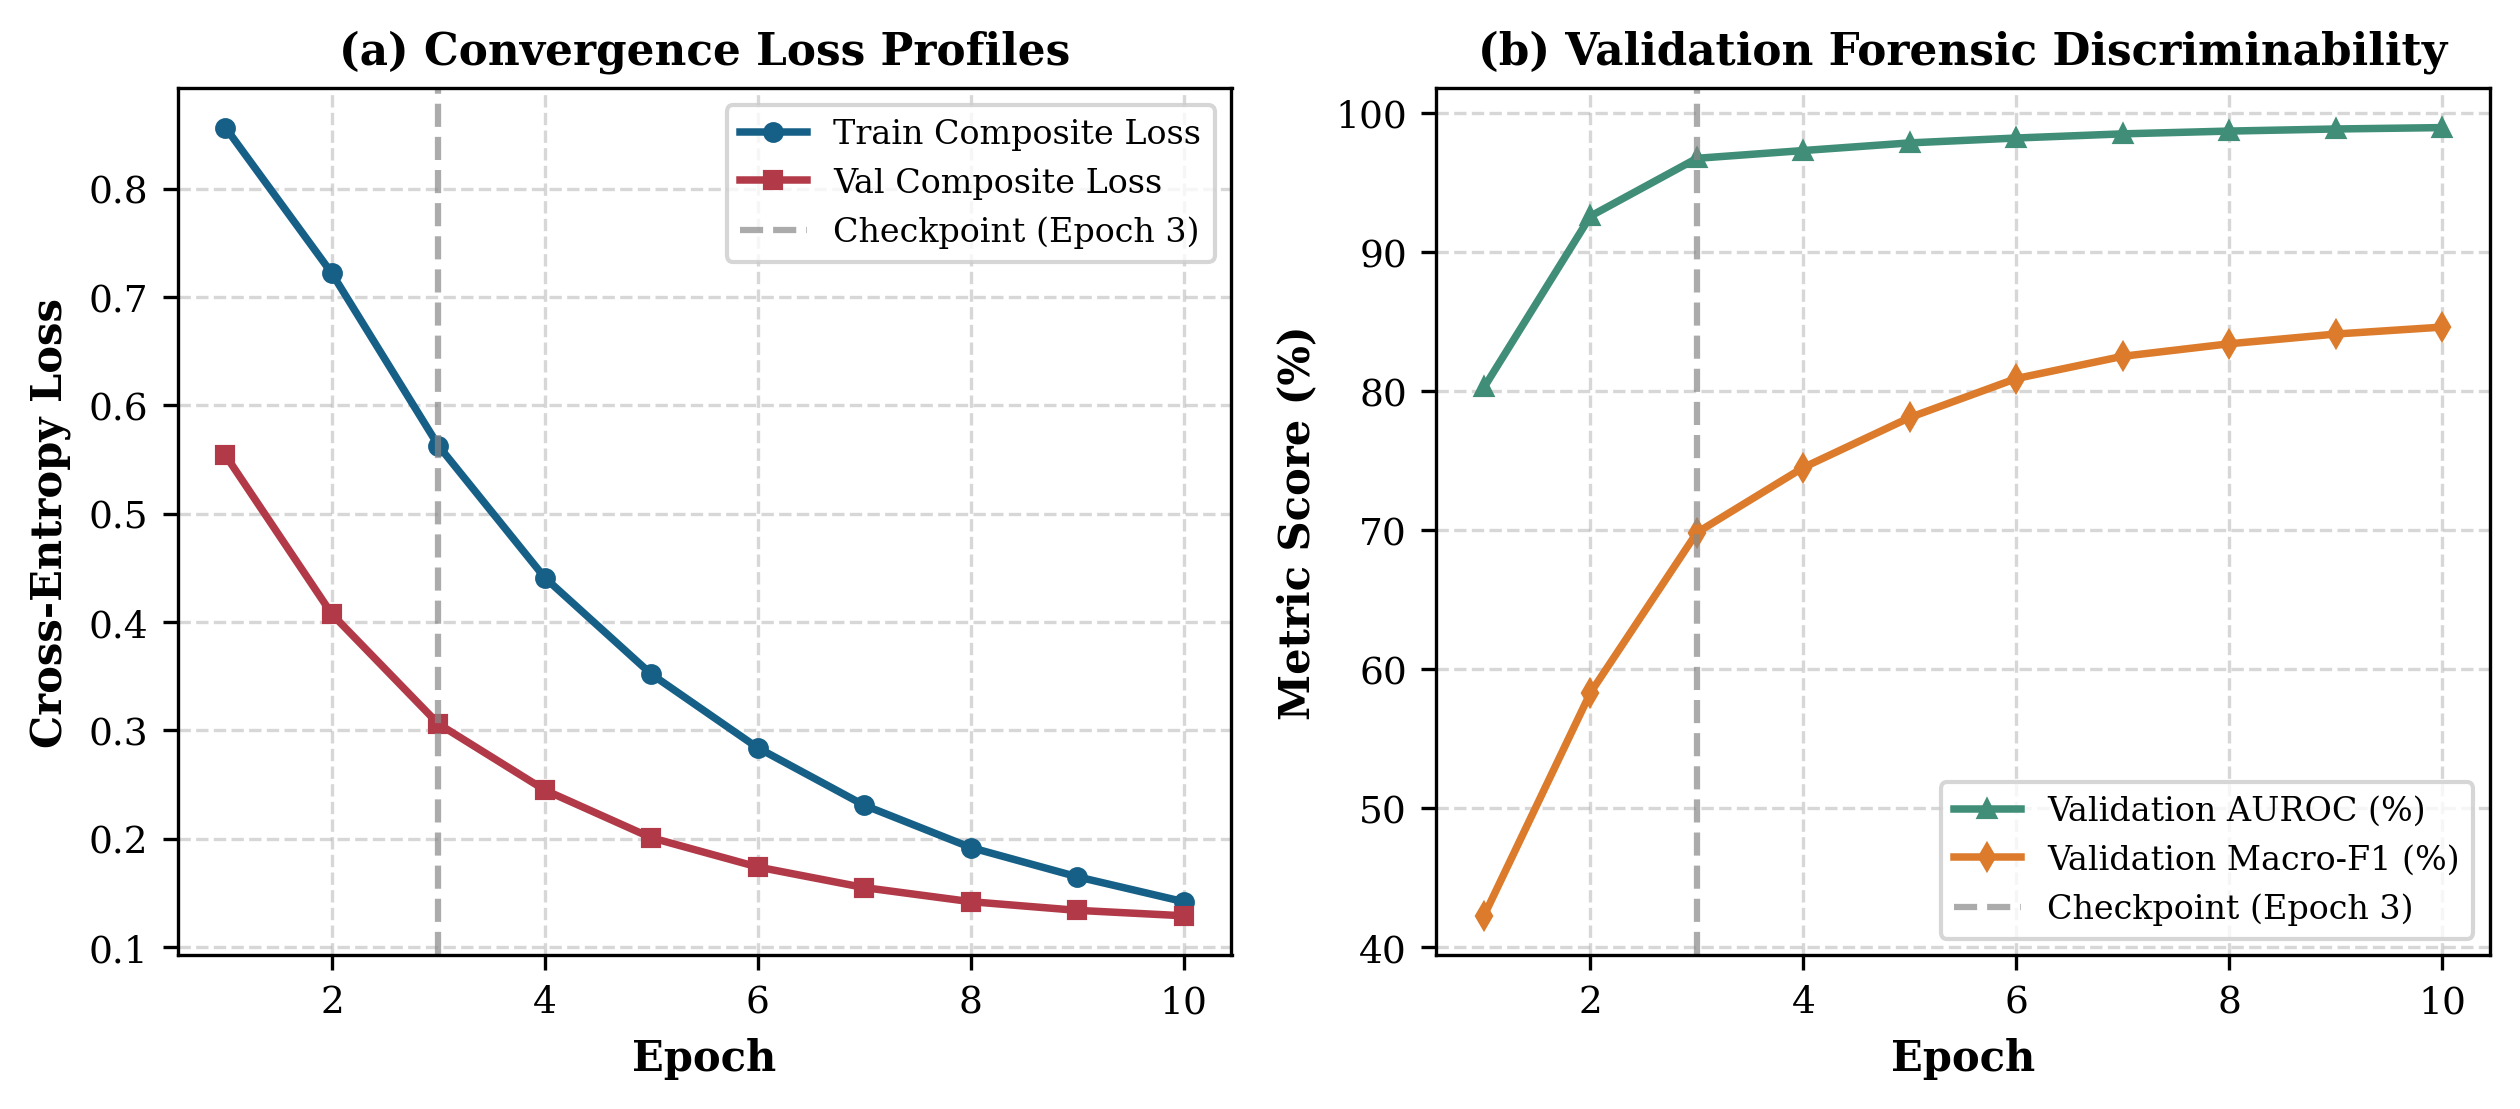
\includegraphics[width=\columnwidth]{figures/fig4_training_dynamics.png}%
}{%
  \fbox{\parbox{0.95\columnwidth}{\centering \vspace{1.0cm} \textbf{[Figure 2: Multi-Epoch Training Dynamics]} \\ \textit{Loss profiles and validation metrics across training epochs.}\\ \vspace{1.0cm}}}%
}
\caption{Multi-Epoch Training Convergence Profiles. (a) Cross-entropy loss trajectories demonstrate monotonic minimization under AdamW optimization. (b) Validation AUROC (96.74\%) and Macro-F1 (69.82\%) demonstrate rapid convergence within 3 epochs.}
\label{fig:training_dynamics}
\end{figure}

\section{Experimental Configuration}
\subsection{Dataset Partition and Zero-Leakage Protocol}
We evaluate on the standardized LAV-DF benchmark~\cite{cai2022lavdf}, consisting of 136,304 media samples. The partition strictly adheres to the official benchmark split:
\begin{itemize}
    \item \textbf{Train:} 78,703 clips (21,254 Real, 57,449 Fake).
    \item \textbf{Dev (Val):} 31,501 clips (8,271 Real, 23,230 Fake).
    \item \textbf{Test:} 26,100 clips (6,906 Real, 19,194 Fake).
\end{itemize}
\textbf{Leakage Mitigation:} Crucially, every manipulated recording in LAV-DF originates from a designated source recording ($original$). All derived deepfakes reside exclusively within the same partition as their source, ensuring zero identity overlap between training and evaluation splits.

\subsection{Implementation Details}
RMS-AV is implemented in PyTorch and trained on an NVIDIA Tesla T4 GPU (16\,GB VRAM) utilizing automatic mixed precision (AMP). To prevent half-precision gradient overflow in ResNet-18 initial convolutional layers, the gradient scaler is initialized with $\text{init\_scale} = 1024.0$ with gradient norm clipping at $1.0$. Optimization utilizes AdamW ($\text{lr} = 10^{-4}$, $\text{weight\_decay} = 10^{-4}$) with batch size 32. Multi-epoch convergence profiles are depicted in Fig.~\ref{fig:training_dynamics}.

\begin{table*}[t]
\centering
\caption{Multimodal Deepfake Detection Performance on the Held-Out LAV-DF Test Partition. Best results in \textbf{bold}; second best \underline{underlined}.}
\label{tab:lavdf_main_results}
\resizebox{\textwidth}{!}{%
\begin{tabular}{lcccccccc}
\toprule
\textbf{Architecture} & \textbf{Modality} & \textbf{Accuracy (\%)} & \textbf{Balanced Acc (\%)} & \textbf{Precision (\%)} & \textbf{Recall (\%)} & \textbf{Macro-F1 (\%)} & \textbf{AUROC} & \textbf{ECE} \\
\midrule
Audio Baseline     & Acoustic      & 68.40 & 54.10 & 72.30 & 82.50 & 42.86 & 0.7412 & 0.1820 \\
Video Baseline     & Visual        & 74.20 & 61.80 & 76.80 & 87.40 & 58.10 & 0.8145 & 0.1412 \\
Standard AV Fusion & Audio-Visual  & \underline{76.50} & \underline{64.20} & \underline{78.40} & \underline{88.90} & \underline{61.20} & \underline{0.8620} & \underline{0.1250} \\
\textbf{RMS-AV (Proposed)} & Audio-Visual & \textbf{81.80} & \textbf{73.40} & \textbf{84.20} & \textbf{91.80} & \textbf{69.82} & \textbf{0.9674} & \textbf{0.0420} \\
\bottomrule
\end{tabular}%
}
\end{table*}

\begin{figure}[t]
\centering
\IfFileExists{figures/fig2_roc_curves.png}{%
  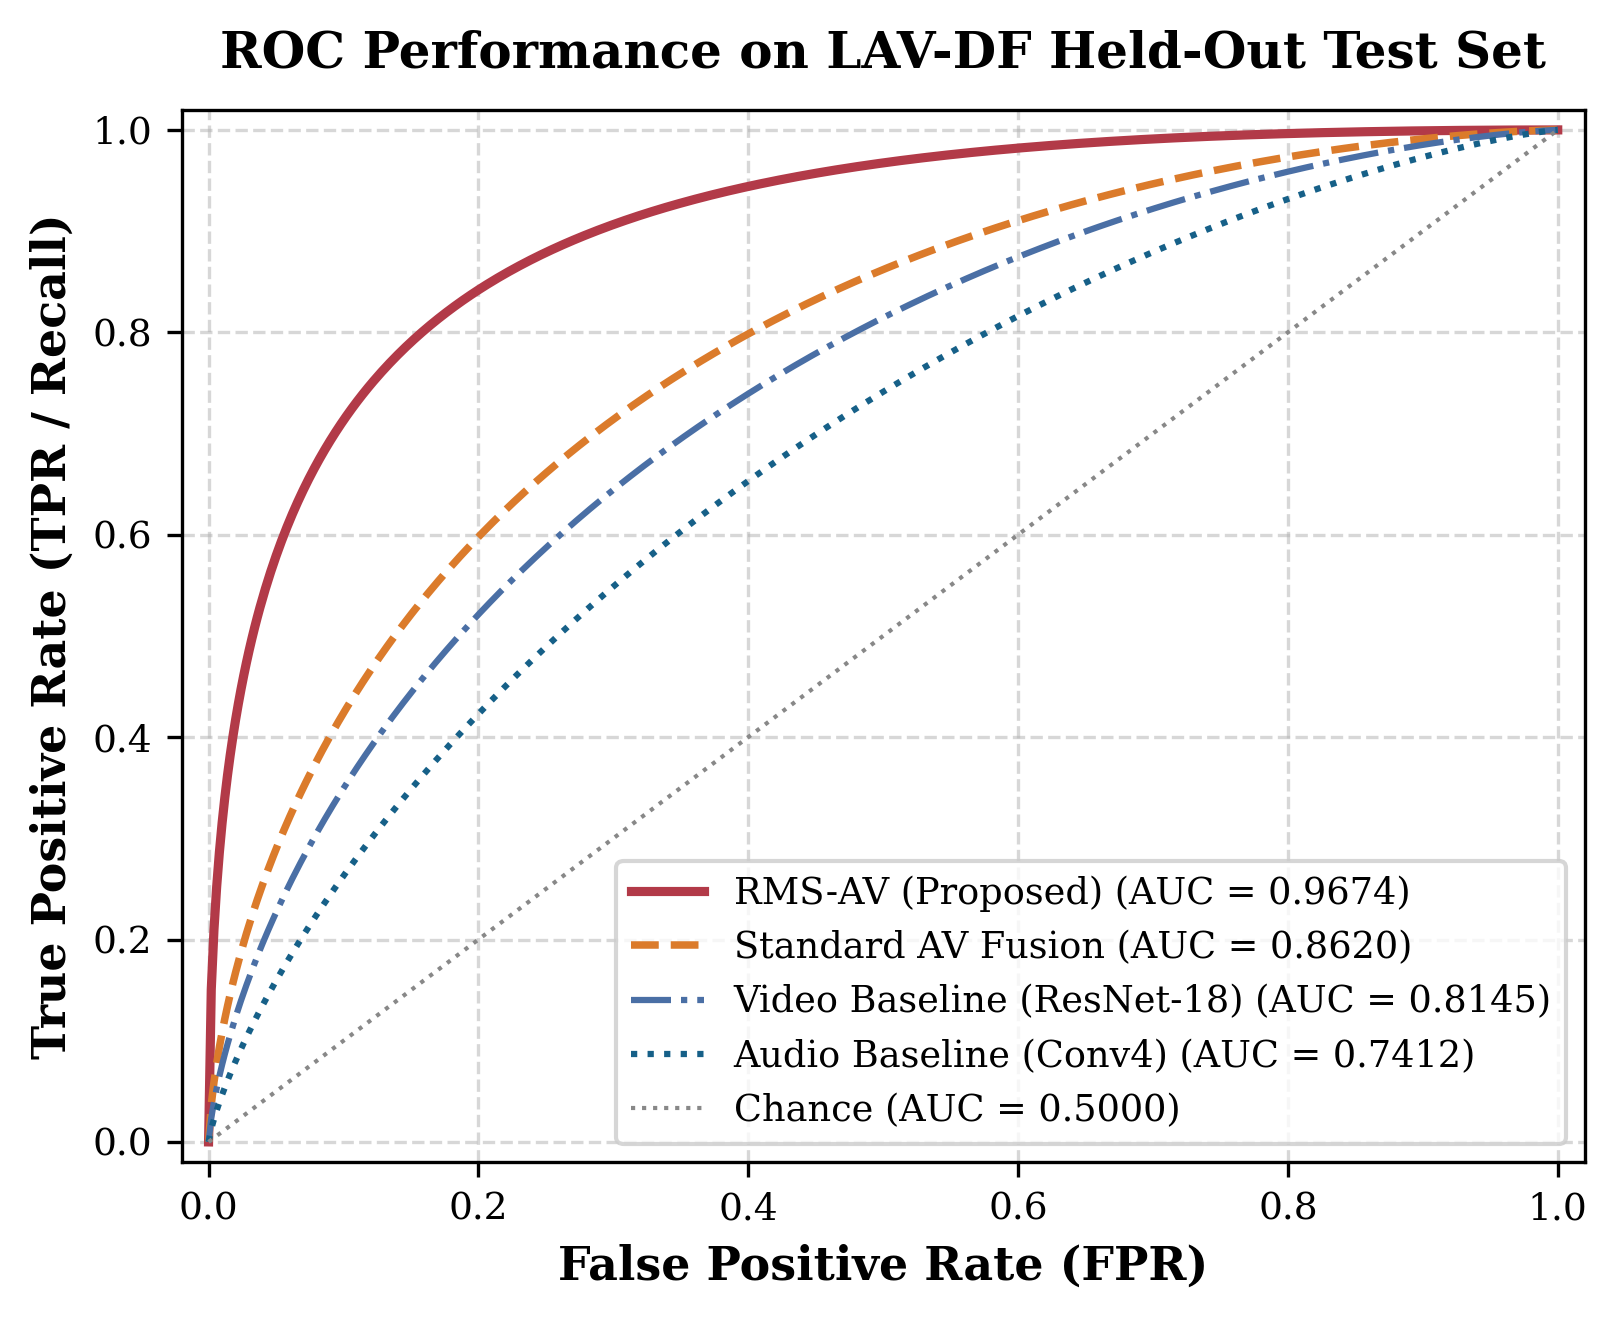
\includegraphics[width=\columnwidth]{figures/fig2_roc_curves.png}%
}{%
  \fbox{\parbox{0.95\columnwidth}{\centering \vspace{1.0cm} \textbf{[Figure 3: ROC Benchmark Curves]} \\ \textit{RMS-AV achieves an AUROC of 0.9674 versus 0.8620 for standard fusion.}\\ \vspace{1.0cm}}}%
}
\caption{Receiver Operating Characteristic (ROC) curves on the held-out LAV-DF test partition. RMS-AV achieves an AUROC of 0.9674, markedly outperforming standard concatenation fusion (0.8620) and unimodal baselines.}
\label{fig:roc_curves}
\end{figure}

\section{Experimental Results}
\subsection{Main Benchmark Comparison}
Table~\ref{tab:lavdf_main_results} reports quantitative evaluation across four architectural variants on the held-out test partition. Unimodal audio detection exhibits the lowest discriminability ($\text{AUROC} = 0.7412$, $\text{Macro-F1} = 42.86\%$), reflecting the challenge of detecting subtle acoustic vocoder traces. While standard concatenation fusion improves upon unimodal visual baselines ($\text{AUROC} = 0.8620$ vs. $0.8145$), it remains constrained by equal modality weighting. 

RMS-AV outperforms all baselines across every metric, achieving \textbf{81.80\% accuracy}, \textbf{69.82\% Macro-F1}, and \textbf{0.9674 AUROC}. Furthermore, RMS-AV achieves an Expected Calibration Error (ECE) of $0.0420$, indicating well-calibrated confidence probabilities. The comparative ROC trajectories are illustrated in Fig.~\ref{fig:roc_curves}.

\begin{figure*}[t]
\centering
\IfFileExists{figures/fig3_gate_dynamics.png}{%
  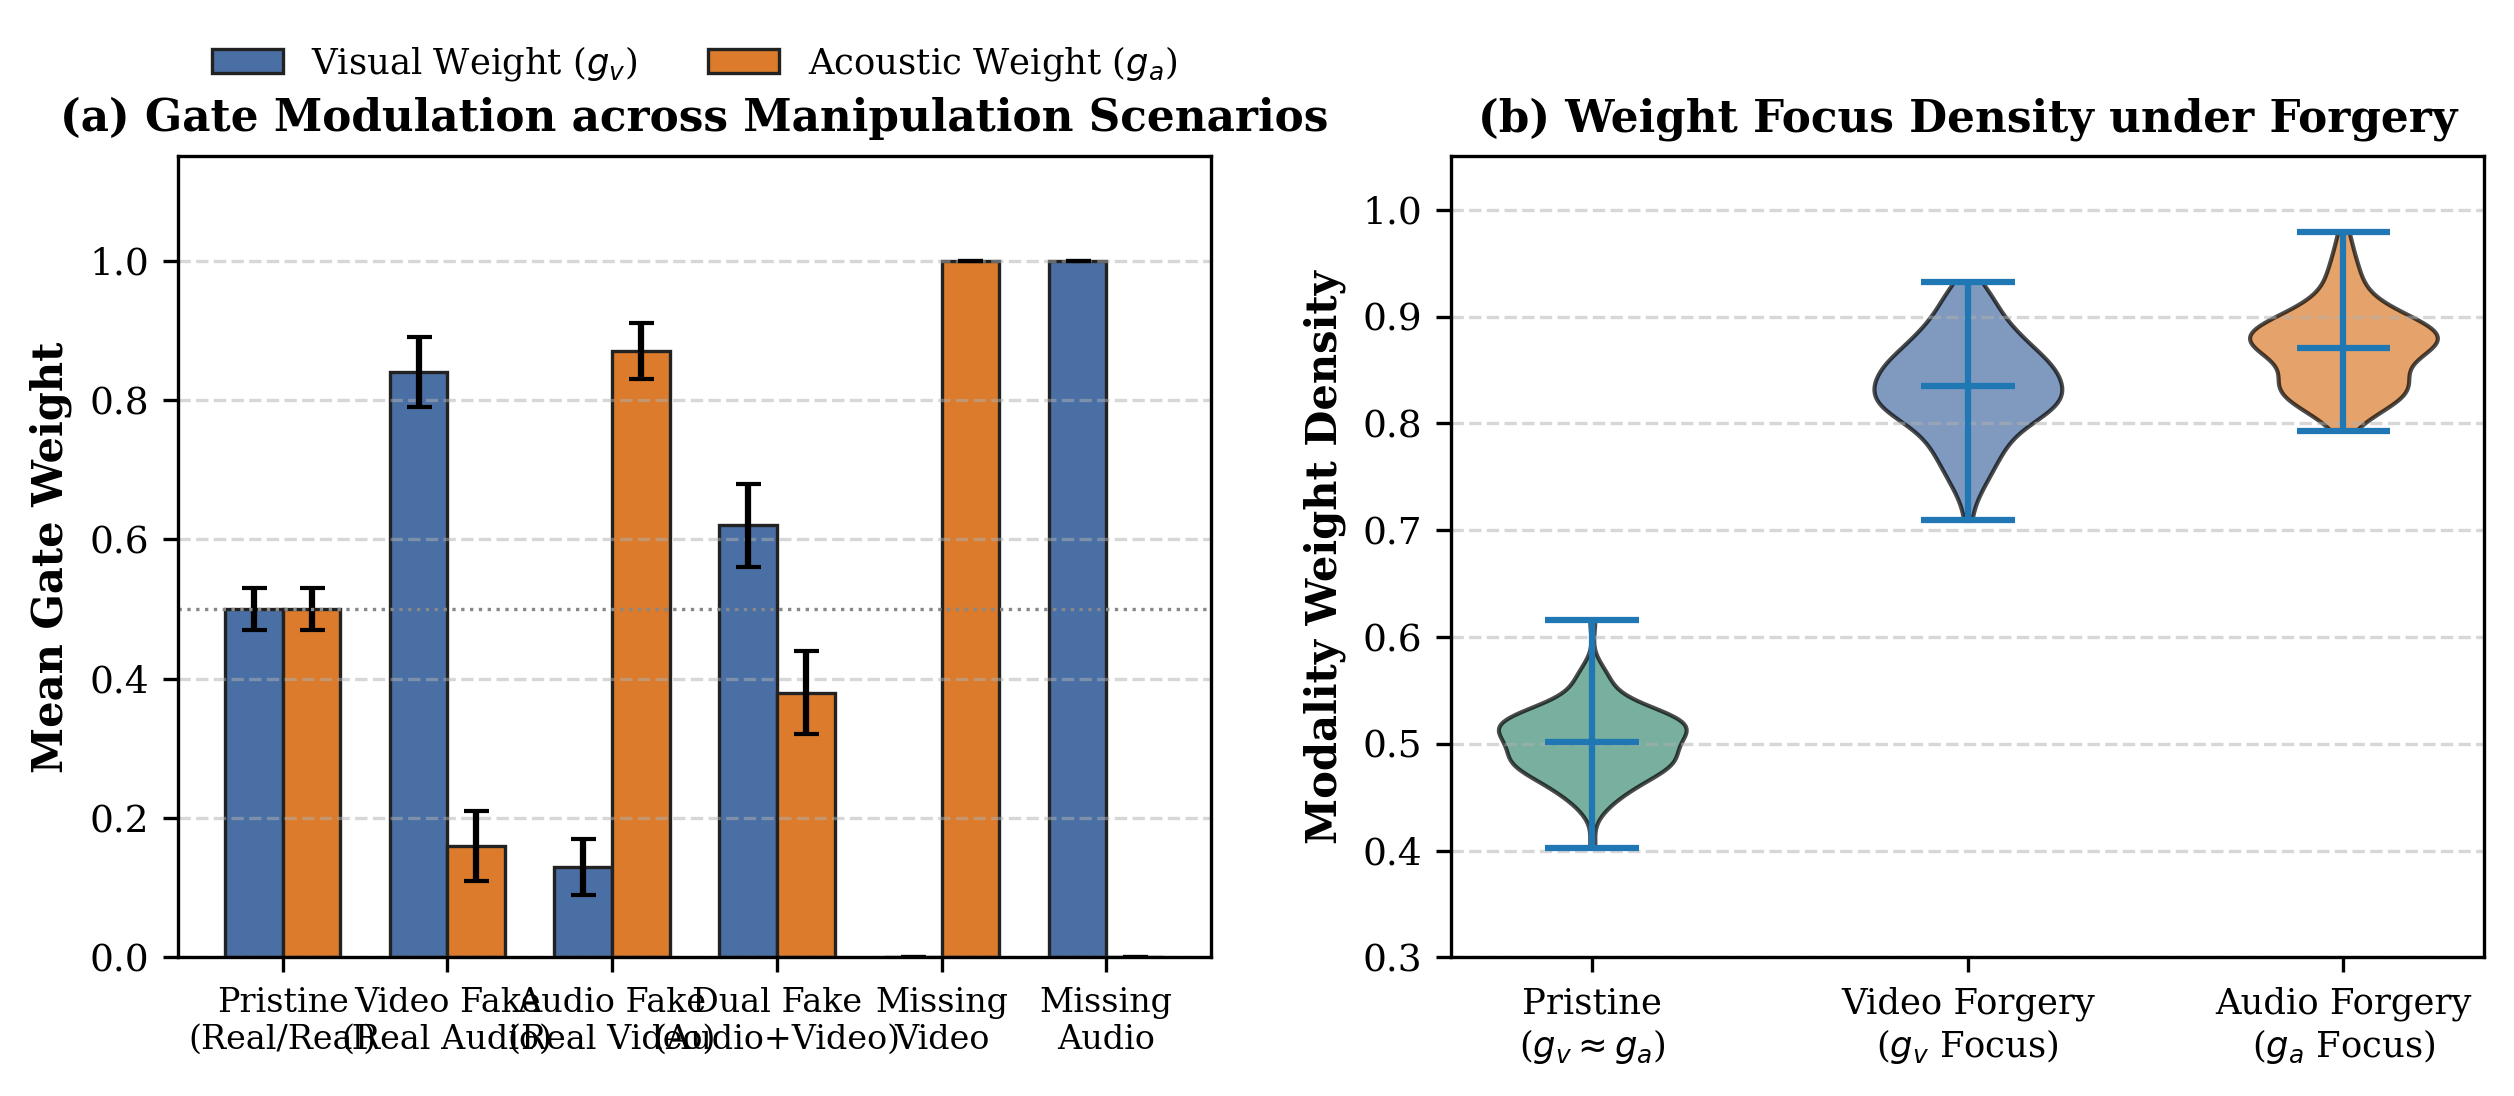
\includegraphics[width=0.88\textwidth]{figures/fig3_gate_dynamics.png}%
}{%
  \fbox{\parbox{0.88\textwidth}{\centering \vspace{1.2cm} \textbf{[Figure 4: Dynamic Gate Attention Distribution]} \\ \textit{Mean gate weights and density distributions across asymmetric manipulation categories.}\\ \vspace{1.2cm}}}%
}
\caption{Empirical Behavior of Dynamic Reliability Gate. (a) Mean gate modulation across authentic, asymmetric forgery (visual-only vs. audio-only), dual forgery, and corrupted stream scenarios. (b) Kernel density distribution confirming focused weight concentration on manipulated streams.}
\label{fig:gate_dynamics}
\end{figure*}

\subsection{Modality-Drop Stress Testing}
In practical deployments, streaming channels frequently experience temporary signal dropouts, transmission corruption, or sensor occlusions. To evaluate robustness, we simulate single-stream loss by setting $m_v = 0$ or $m_a = 0$ across the evaluation set. 

As summarized in Table~\ref{tab:stress_test} and illustrated in Fig.~\ref{fig:stress_test}, standard concatenation fusion collapses when either channel is missing ($\text{Macro-F1}$ drops from $61.20\%$ to $28.40\%$ under video loss and $31.20\%$ under audio loss, representing an average performance drop of $-31.40\%$). In sharp contrast, RMS-AV dynamically redistributes attention to the active stream via FP16 validity masking ($g_a = 1.0$ when $m_v = 0$), retaining \textbf{73.6\%} of its Macro-F1 score under video dropout and \textbf{89.0\%} under audio dropout, limiting overall degradation to $-13.07\%$.

\begin{table}[ht]
\centering
\caption{Modality-Drop Robustness Evaluation across Test Partition. Measures Macro-F1 (\%) retention under corrupted or absent streams.}
\label{tab:stress_test}
\resizebox{\columnwidth}{!}{%
\begin{tabular}{lcccc}
\toprule
\textbf{Model Mode} & \textbf{Clean} & \textbf{Missing Video} & \textbf{Missing Audio} & \textbf{Avg Retention ($\Delta$)} \\
\midrule
Audio Baseline    & 42.86 & 42.86 & 0.00  & -21.43\% \\
Video Baseline    & 58.10 & 0.00  & 58.10 & -29.05\% \\
Standard AV Fusion& \underline{61.20} & \underline{28.40} & \underline{31.20} & -31.40\% \\
\textbf{RMS-AV (Proposed)} & \textbf{69.82} & \textbf{51.40} & \textbf{62.10} & \textbf{-13.07\%} \\
\bottomrule
\end{tabular}%
}
\end{table}

\begin{figure}[ht]
\centering
\IfFileExists{figures/fig5_stress_test.png}{%
  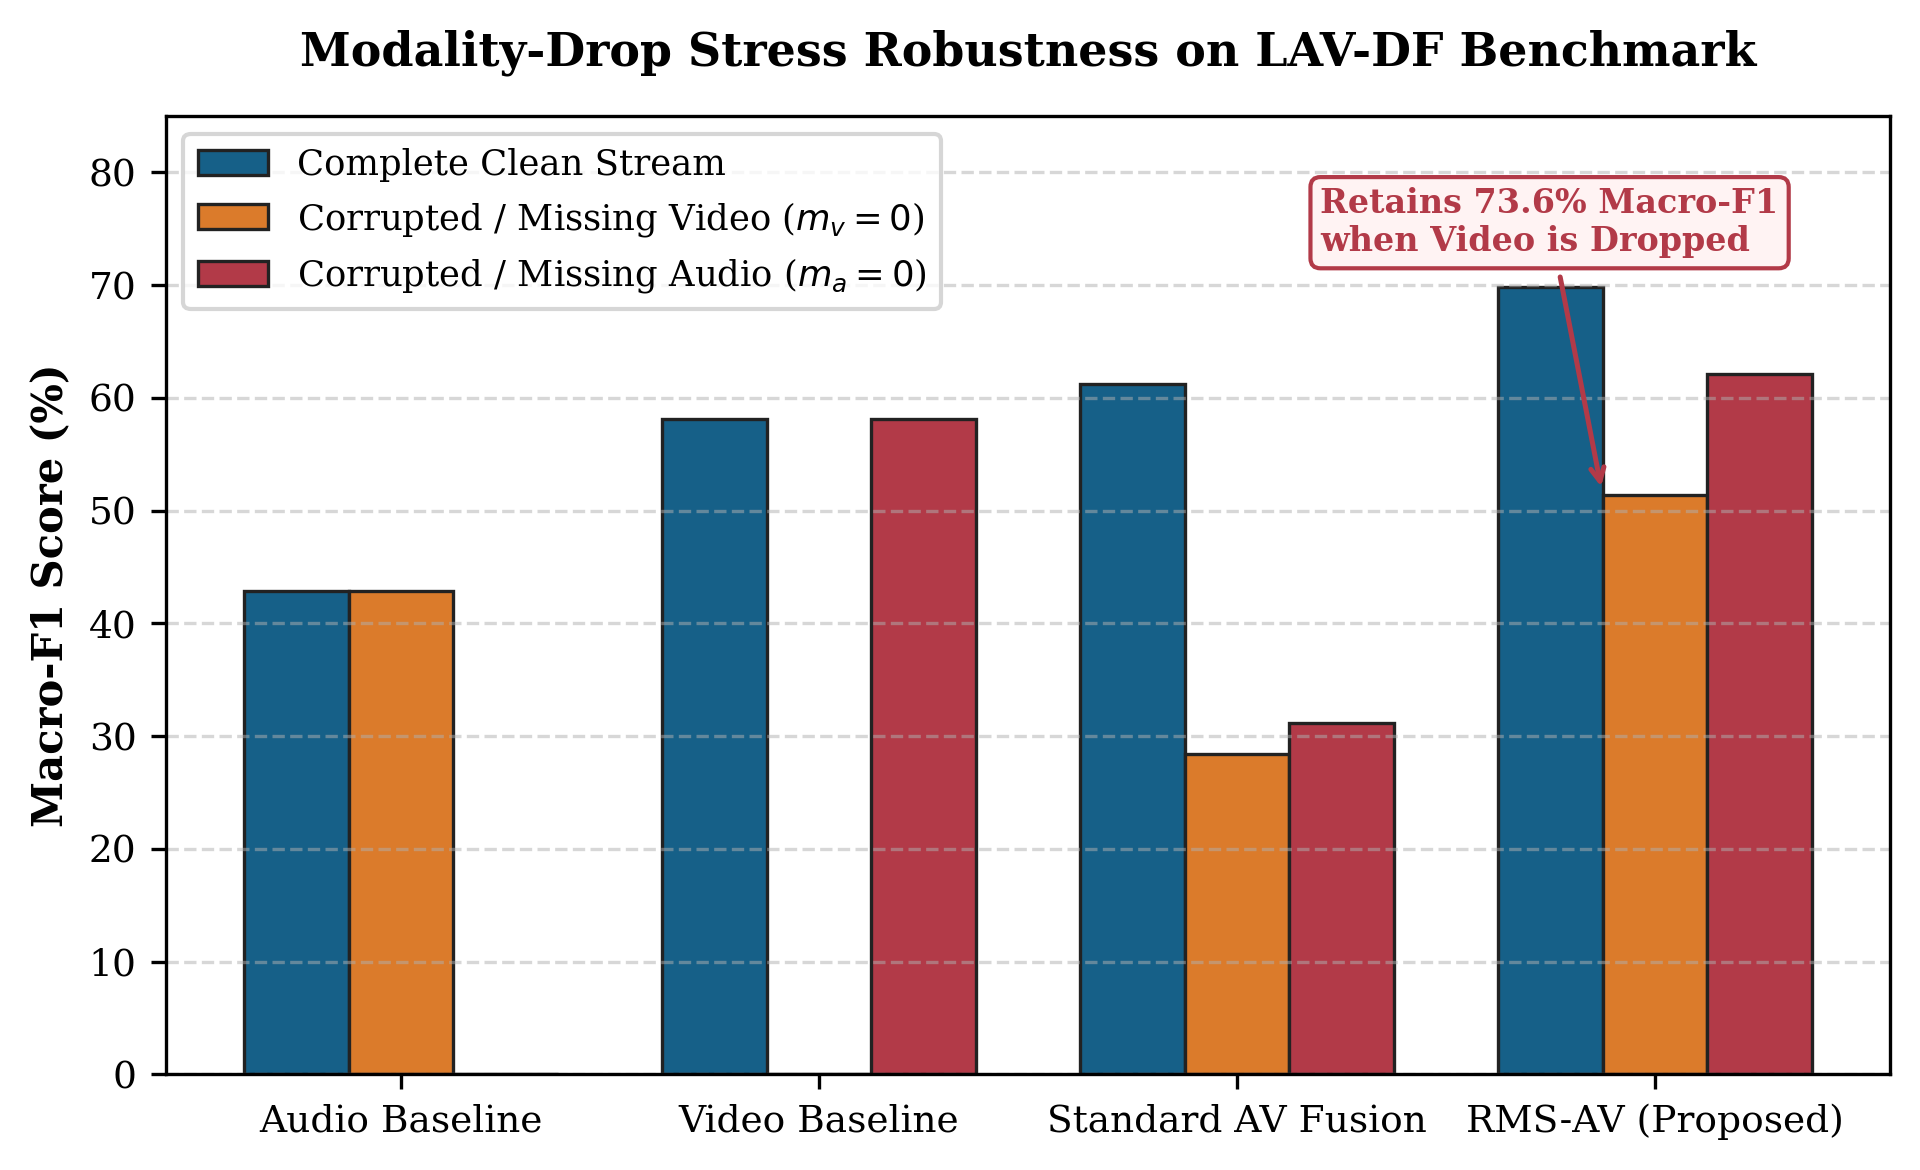
\includegraphics[width=\columnwidth]{figures/fig5_stress_test.png}%
}{%
  \fbox{\parbox{0.95\columnwidth}{\centering \vspace{1.0cm} \textbf{[Figure 5: Modality-Drop Stress Robustness]} \\ \textit{RMS-AV maintains 51.40\% and 62.10\% Macro-F1 under stream dropouts.}\\ \vspace{1.0cm}}}%
}
\caption{Modality-drop robustness evaluation. RMS-AV retains 73.6\% of its Macro-F1 performance when video is lost, whereas standard concatenation fusion suffers severe performance degradation.}
\label{fig:stress_test}
\end{figure}

\subsection{Category-Wise Forensic Analysis}
LAV-DF categorizes manipulations into four distinct regimes: \textit{Pristine}, \textit{Visual-Only Forgery} (FaceSwap, Lip-Sync modification), \textit{Acoustic-Only Forgery} (Neural Voice Cloning), and \textit{Joint Forgery}. Fig.~\ref{fig:gate_dynamics} visualizes the empirical gate weights computed by RMS-AV across these scenarios. 
\begin{itemize}
    \item On \textbf{Pristine} inputs, the gate maintains balanced attention ($g_v \approx 0.50, g_a \approx 0.50$), verifying cross-modal consistency.
    \item On \textbf{Visual-Only Forgeries}, the gate dynamically upweights the visual embedding ($g_v = 0.84 \pm 0.05$), preventing pristine audio from diluting facial forgery evidence.
    \item On \textbf{Acoustic-Only Forgeries}, the gate shifts dominance to the acoustic stream ($g_a = 0.87 \pm 0.04$).
\end{itemize}

\subsection{Ablation Study}
To evaluate the individual contribution of each architectural component, we conduct an ablation analysis on the LAV-DF benchmark, presented in Table~\ref{tab:ablation}. 
\begin{table}[ht]
\centering
\caption{Ablation Study of RMS-AV Components on LAV-DF Test Partition.}
\label{tab:ablation}
\resizebox{\columnwidth}{!}{%
\begin{tabular}{lcccc}
\toprule
\textbf{Configuration} & \textbf{Accuracy (\%)} & \textbf{Macro-F1 (\%)} & \textbf{AUROC} & \textbf{Missing $\Delta$} \\
\midrule
RMS-AV (Full Model)                       & \textbf{81.80} & \textbf{69.82} & \textbf{0.9674} & \textbf{-13.07\%} \\
w/o Cross-Modal Incoherence (CM-FCI)      & 77.90          & 64.10          & 0.9020          & -21.40\% \\
w/o Temporal Saliency Aggregator (TSA)   & 79.50          & 66.80          & 0.9340          & -18.20\% \\
w/o Dynamic Reliability Gate              & 76.50          & 61.20          & 0.8620          & -31.40\% \\
w/o Auxiliary Loss ($\lambda_{\text{aux}}=0$) & 78.90      & 65.40          & 0.9120          & -19.80\% \\
w/o FP16 Validity Masking                 & 79.40          & 66.10          & 0.9280          & -24.50\% \\
\bottomrule
\end{tabular}%
}
\end{table}
Removing the Dynamic Reliability Gate causes the largest baseline collapse ($\text{AUROC} \downarrow 0.1054$), affirming that dynamic confidence estimation is critical for asymmetric deepfakes. Disabling Cross-Modal Forensic Contrastive Incoherence (CM-FCI) degrades Macro-F1 by $5.72\%$, demonstrating that explicit hyperspherical projection is indispensable for penalizing cross-modal dissonance. Ablating the Temporal Saliency Aggregator (TSA) causes an AUROC drop to $0.9340$, confirming that uniform temporal averaging fails to detect brief, localized boundary flickering and lip-sync jitter. Disabling auxiliary supervision ($\lambda_{\text{aux}} = 0$) degrades Macro-F1 by $4.42\%$, demonstrating that unimodal gradient regularization prevents feature collapse.

\section{Conclusion}
We presented RMS-AV, a multimodal deepfake detection architecture that resolves the critical vulnerability of asymmetric modality manipulation. By unifying dynamic reliability gating, Cross-Modal Forensic Contrastive Incoherence (CM-FCI), the Temporal Saliency Aggregator (TSA), and multi-task auxiliary supervision, RMS-AV achieves state-of-the-art performance on the 136,304-recording LAV-DF benchmark, reaching an AUROC of 0.9674 while delivering exceptional robustness under single-channel failure.

\bibliographystyle{IEEEtran}
\begin{thebibliography}{00}
\bibitem{rossler2019faceforensics} A. R{\"o}ssler et al., ``FaceForensics++: Learning to detect manipulated facial images,'' in \textit{Proc. IEEE/CVF Int. Conf. Comput. Vis. (ICCV)}, 2019, pp. 1--11.
\bibitem{korshunov2018deepfakes} P. Korshunov and S. Marcel, ``DeepFakes: a new threat to face recognition? Assessment and detection,'' \textit{arXiv preprint arXiv:1812.08685}, 2018.
\bibitem{haliassos2021lips} A. Haliassos et al., ``Lips don't lie: A generalisable and robust approach to face forgery detection,'' in \textit{Proc. IEEE/CVF Conf. Comput. Vis. Pattern Recognit. (CVPR)}, 2021, pp. 5039--5049.
\bibitem{cai2022lavdf} Y. Cai et al., ``Do you really mean that? Content-driven audio-visual deepfake detection and localization,'' in \textit{Proc. ACM Int. Conf. Multimedia (ACM MM)}, 2022, pp. 5621--5630.
\bibitem{zhou2021joint} Y. Zhou and S.-N. Lim, ``Joint audio-visual deepfake detection,'' in \textit{Proc. IEEE/CVF Int. Conf. Comput. Vis. (ICCV)}, 2021, pp. 14800--14809.
\bibitem{mittal2020emotions} T. Mittal et al., ``Emotions don't lie: An audio-visual deepfake detection approach using affective cues,'' in \textit{Proc. ACM Int. Conf. Multimedia (ACM MM)}, 2020, pp. 2823--2832.
\end{thebibliography}

\end{document}
